
% \documentclass[11pt,a4paper]{article}
\documentclass{report}



% Page Layout
\usepackage[tmargin=2cm,rmargin=1in,lmargin=1in,margin=0.85in,bmargin=2cm,footskip=0.0in]{geometry}
% Controls page margins, text width/height, footskip, etc.

\setlength{\parindent}{0pt}      % no paragraph indent
\setlength{\parskip}{0.4em}      % small, consistent gap between paragraphs


% 📚 Math & Symbols
\usepackage{amsmath,amsfonts,amsthm,amssymb,mathtools,bbm,bm}
% Core AMS math tools (theorems, align, fonts, symbols).

% bbm – Provides blackboard bold \mathbbm{1} indicator symbol.
% bm – Bold math symbols (\bm{x}).
% newpxmath – Times-like math font compatible with Palatino/PX fonts.
% xfrac – Inline slanted fractions using \sfrac{a}{b}.
% cancel – Strikeout terms in equations with \cancel{}.
\usepackage[varbb]{newpxmath}

\usepackage{xfrac}
\usepackage[makeroom]{cancel}
\usepackage{mathtools}



% 🔗 Navigation & References
\usepackage{bookmark} % Improved handling of PDF bookmarks.
\usepackage{hyperref,theoremref} 
% Allows references like “Theorem 1.2”.
\usepackage{nameref} 
% Reference by section name (\nameref{section}).



% 📦 Layout, Lists, Tables
\usepackage{enumitem} % Customize list spacing and labels
\usepackage{multicol,array} 
% multicol – Multiple column layout inside the page.
% array – Enhanced tabular column features.



% 🎨 Graphics & Coloring
\usepackage{xcolor} % Colored text and drawing.
\usepackage{tikz-cd} % Commutative diagrams (TikZ-based).
\usepackage{transparent} % Adjust text/image transparency.
% \usepackage[most]{tcolorbox}


% 📑 Frames, Boxes, and Visual Elements
\usepackage[most,many,breakable]{tcolorbox}
% Colored/fancy boxes, breakable boxes, theorems.
\usepackage{varwidth} % Boxes with variable width (auto-fit content)
% <<< PUT IT RIGHT HERE >>>
\tcbset{fontupper=\normalsize}


% 🔧 Utilities & Tools
\usepackage{etoolbox}
% Logic programming tools (patching commands, conditionals).
\usepackage{xifthen} 
% Conditional statements (\ifthenelse) with logic.
\usepackage{import}
% Import figures or files from subdirectories.
\usepackage{pdfpages}
% Insert external PDF pages (\includepdf).
\usepackage{comment} 
% Multi-line comment environment.
\usepackage[ruled,vlined,linesnumbered]{algorithm2e}
% Nice-looking algorithm environment (algorithm2e).
\usepackage{natbib}
% Author–year and numeric citation management (needed for JFE, JFQA styles).

\usepackage{tikz}
\usetikzlibrary{positioning}
\usepackage{tikzsymbols}
\renewcommand\qedsymbol{$\Laughey$}

% the package for the table
% \usepackage{booktabs}
% \usepackage{threeparttable}
\usepackage{multirow}
% \usepackage{adjustbox}
\usepackage{tabularx}
\newcolumntype{Y}{>{\raggedleft\arraybackslash}X}


% minted is a LaTeX package for beautifully formatting source code with syntax highlighting.
% \usepackage{minted}
% \definecolor{LightGray}{gray}{0.95}

% \hypersetup{
% 	pdftitle={Notes},
% 	colorlinks=true, linkcolor=blue,
% 	bookmarksnumbered=true,
% 	bookmarksopen=true
% }

% \hypersetup{
%     pdftitle={PhD Research Notes},
%     colorlinks=true,
%     linkcolor=blue!50!black,
%     citecolor=blue!50!black,
%     urlcolor=blue!70!black,
%     bookmarksnumbered=true,
%     bookmarksopen=true
% }

% \hypersetup{
%     pdftitle={PhD Research Notes},
%     colorlinks=true,
%     linkcolor=blue,
%     citecolor=blue,
%     urlcolor=blue,
%     bookmarksnumbered=true,
%     bookmarksopen=true
% }

% Original hyper set up
\hypersetup{
	pdftitle={Assignment},
	colorlinks=true, linkcolor=doc!90,
	bookmarksnumbered=true,
	bookmarksopen=true
}

% Nice tables
\usepackage{booktabs}        % \toprule \midrule \bottomrule
\usepackage{threeparttable}  % notes under tables
\usepackage{siunitx}         % numeric alignment
\usepackage{adjustbox}       % resize table to fit width
\usepackage{caption}         % caption styling (optional)

% draw figure in latex
\usepackage{tikz}
\usetikzlibrary{arrows.meta, positioning, shapes.geometric}


% siunitx setup: adjust to your taste
\sisetup{
  detect-all,
  input-symbols   = (),
  table-number-alignment = center,
  group-separator = {,},
  group-minimum-digits = 4,
  table-space-text-post = ***,
}

% slightly tighter / nicer table spacing
\setlength{\tabcolsep}{6pt}
\renewcommand{\arraystretch}{1.15}


% %%%%%%%%%%%%%%%%%%%%%%%%%%%%%%
% % SELF MADE COLORS
% %%%%%%%%%%%%%%%%%%%%%%%%%%%%%%



\definecolor{myg}{RGB}{56, 140, 70}
\definecolor{myb}{RGB}{45, 111, 177}
% \definecolor{myr}{RGB}{199, 68, 64}
\definecolor{mytheorembg}{HTML}{F2F2F9}
\definecolor{mytheoremfr}{HTML}{00007B}
% \definecolor{mylenmabg}{HTML}{FFFAF8}
% \definecolor{mylenmafr}{HTML}{983b0f}
% \definecolor{mypropbg}{HTML}{f2fbfc}
% \definecolor{mypropfr}{HTML}{191971}
\definecolor{myexamplebg}{HTML}{F2FBF8}
\definecolor{myexamplefr}{HTML}{88D6D1}
\definecolor{myexampleti}{HTML}{2A7F7F}
% \definecolor{mydefinitbg}{HTML}{E5E5FF}
% \definecolor{mydefinitfr}{HTML}{3F3FA3}
% \definecolor{notesgreen}{RGB}{0,162,0}
\definecolor{myp}{RGB}{197, 92, 212}
\definecolor{mygr}{HTML}{2C3338}
\definecolor{myred}{RGB}{127,0,0}
\definecolor{myyellow}{RGB}{169,121,69}
% \definecolor{myexercisebg}{HTML}{F2FBF8}
% \definecolor{myexercisefg}{HTML}{88D6D1}

\definecolor{softredbg}{RGB}{255,235,238}   % very light, soft red background
\definecolor{softredline}{RGB}{198,40,40}   % deep soft red for the border/title
\definecolor{softbluebg}{RGB}{232,245,253}   % very light soft-blue background
\definecolor{softblueline}{RGB}{30,136,229}  % soft but strong blue (border/title)
\definecolor{softgreybg}{RGB}{245,245,245}   % very light grey background
\definecolor{softgreyline}{RGB}{150,150,150} % medium grey border/title


% =====================================================
%  COLOR PALETTE FOR READING NOTES
% =====================================================
\definecolor{refabg}{RGB}{232,245,233}   % soft blue     (Abstract)
\definecolor{refaline}{RGB}{56,142,60}

\definecolor{refmbg}{RGB}{232,245,253}   % soft green    (Method)
\definecolor{refmline}{RGB}{30,136,229}

\definecolor{refcbg}{RGB}{255,235,238}   % soft red   (Conclusion)
\definecolor{refcline}{RGB}{198,40,40}

\definecolor{reflbg}{RGB}{255,249,230}   % soft yellow   (Background/Literature)
\definecolor{reflline}{RGB}{251,192,45}

\definecolor{refnote_bg}{RGB}{245,245,245}   % soft grey (Your comments)
\definecolor{refnote_line}{RGB}{120,120,120}

\tcbuselibrary{skins,breakable}

% =====================================================
% 1. ABSTRACT BOX
% =====================================================
\newtcolorbox{refabstract}[1][]{%
  enhanced, breakable,
  colback=refabg,
  colframe=refaline,
  boxrule=0.8pt,
  borderline west={2pt}{0pt}{refaline},
  sharp corners,
  title=\textbf{Abstract},
  coltitle=refaline,
  fonttitle=\bfseries\sffamily,
  detach title,
  before upper=\tcbtitle\par\smallskip,
  #1
}

% =====================================================
% 2. METHODOLOGY BOX
% =====================================================
\newtcolorbox{refmethod}[1][]{%
  enhanced, breakable,
  colback=refmbg,
  colframe=refmline,
  boxrule=0.8pt,
  borderline west={2pt}{0pt}{refmline},
  sharp corners,
  title=\textbf{Methodology},
  coltitle=refmline,
  fonttitle=\bfseries\sffamily,
  detach title,
  before upper=\tcbtitle\par\smallskip,
  #1
}

% =====================================================
% 3. KEY FINDINGS / CONCLUSION BOX
% =====================================================
\newtcolorbox{refconclusion}[1][]{%
  enhanced, breakable,
  colback=refcbg,
  colframe=refcline,
  boxrule=0.8pt,
  borderline west={2pt}{0pt}{refcline},
  sharp corners,
  title=\textbf{Key Findings / Conclusion},
  coltitle=refcline,
  fonttitle=\bfseries\sffamily,
  detach title,
  before upper=\tcbtitle\par\smallskip,
  #1
}

% =====================================================
% 4. BACKGROUND / LITERATURE / MOTIVATION BOX
% =====================================================
\newtcolorbox{reflitnote}[1][]{%
  enhanced, breakable,
  colback=reflbg,
  colframe=reflline,
  boxrule=0.8pt,
  borderline west={2pt}{0pt}{reflline},
  sharp corners,
  title=\textbf{Background / Literature},
  coltitle=reflline,
  fonttitle=\bfseries\sffamily,
  detach title,
  before upper=\tcbtitle\par\smallskip,
  #1
}

% =====================================================
% 5. YOUR OWN COMMENTS / CRITIQUE BOX
% =====================================================
\newtcolorbox{refcomment}[1][]{%
  enhanced, breakable,
  colback=refnote_bg,
  colframe=refnote_line,
  boxrule=0.8pt,
  borderline west={2pt}{0pt}{refnote_line},
  sharp corners,
  title=\textbf{My Comments},
  coltitle=refnote_line,
  fonttitle=\bfseries\sffamily,
  detach title,
  before upper=\tcbtitle\par\smallskip,
  #1
}


\newtcbox{\mybox}[1][red]{on line,
arc=0pt,outer arc=0pt,colback=#1!10!white,colframe=#1!50!black,
boxsep=0pt,left=1pt,right=1pt,top=2pt,bottom=2pt,
boxrule=0pt,bottomrule=1pt,toprule=1pt}
\newtcbox{\xmybox}[1][red]{on line,
arc=7pt,colback=#1!10!white,colframe=#1!50!black,
before upper={\rule[-3pt]{0pt}{10pt}},boxrule=1pt,
boxsep=0pt,left=6pt,right=6pt,top=2pt,bottom=2pt}


%================================
% EXAMPLE BOX
%================================

\newtcbtheorem[number within=section]{Example}{Example}
{%
	colback = myexamplebg
	,breakable
	,colframe = myexamplefr
	,coltitle = myexampleti
	,boxrule = 1pt
	,sharp corners
	,detach title
	,before upper=\tcbtitle\par\smallskip
	,fonttitle = \bfseries
	,description font = \mdseries
	,separator sign none
	,description delimiters parenthesis
}
{ex}

\newtcbtheorem[number within=chapter]{example}{Example}
{%
	colback = myexamplebg
	,breakable
	,colframe = myexamplefr
	,coltitle = myexampleti
	,boxrule = 1pt
	,sharp corners
	,detach title
	,before upper=\tcbtitle\par\smallskip
	,fonttitle = \bfseries
	,description font = \mdseries
	,separator sign none
	,description delimiters parenthesis
}
{ex}


%================================
% Question BOX
%================================

\makeatletter
\newtcbtheorem{question}{Question}{enhanced,
	breakable,
	colback=white,
	colframe=myb!80!black,
	attach boxed title to top left={yshift*=-\tcboxedtitleheight},
	fonttitle=\bfseries,
	title={#2},
	boxed title size=title,
	boxed title style={%
			sharp corners,
			rounded corners=northwest,
			colback=tcbcolframe,
			boxrule=0pt,
		},
	underlay boxed title={%
			\path[fill=tcbcolframe] (title.south west)--(title.south east)
			to[out=0, in=180] ([xshift=5mm]title.east)--
			(title.center-|frame.east)
			[rounded corners=\kvtcb@arc] |-
			(frame.north) -| cycle;
		},
	#1
}{def}
\makeatother



%================================
% SOLUTION BOX
%================================

\makeatletter
\newtcolorbox{solution}{enhanced,
	breakable,
	colback=white,
	colframe=myg!80!black,
	attach boxed title to top left={yshift*=-\tcboxedtitleheight},
	title=Solution,
	boxed title size=title,
	boxed title style={%
			sharp corners,
			rounded corners=northwest,
			colback=tcbcolframe,
			boxrule=0pt,
		},
	underlay boxed title={%
			\path[fill=tcbcolframe] (title.south west)--(title.south east)
			to[out=0, in=180] ([xshift=5mm]title.east)--
			(title.center-|frame.east)
			[rounded corners=\kvtcb@arc] |-
			(frame.north) -| cycle;
		},
}
\makeatother

% %================================
% % Question BOX
% %================================

% \makeatletter
% \newtcbtheorem{qstion}{Question}{enhanced,
% 	breakable,
% 	colback=white,
% 	colframe=mygr,
% 	attach boxed title to top left={yshift*=-\tcboxedtitleheight},
% 	fonttitle=\bfseries,
% 	title={#2},
% 	boxed title size=title,
% 	boxed title style={%
% 			sharp corners,
% 			rounded corners=northwest,
% 			colback=tcbcolframe,
% 			boxrule=0pt,
% 		},
% 	underlay boxed title={%
% 			\path[fill=tcbcolframe] (title.south west)--(title.south east)
% 			to[out=0, in=180] ([xshift=5mm]title.east)--
% 			(title.center-|frame.east)
% 			[rounded corners=\kvtcb@arc] |-
% 			(frame.north) -| cycle;
% 		},
% 	#1
% }{def}
% \makeatother

% \newtcbtheorem[number within=chapter]{wconc}{Wrong Concept}{
% 	breakable,
% 	enhanced,
% 	colback=white,
% 	colframe=myr,
% 	arc=0pt,
% 	outer arc=0pt,
% 	fonttitle=\bfseries\sffamily\large,
% 	colbacktitle=myr,
% 	attach boxed title to top left={},
% 	boxed title style={
% 			enhanced,
% 			skin=enhancedfirst jigsaw,
% 			arc=3pt,
% 			bottom=0pt,
% 			interior style={fill=myr}
% 		},
% 	#1
% }{def}

% %%%%%%%%%%%%%%%%%%%%%%%%%%%%
% % TCOLORBOX SETUPS
% %%%%%%%%%%%%%%%%%%%%%%%%%%%%

\setlength{\parindent}{0pt}

%================================
% Brainteasers
%================================

\tcbuselibrary{theorems,skins,hooks}
\newtcbtheorem[number within=section]{brainteasers}{Brainteasers}
{%
	enhanced
	,breakable
	,colback = myg!10
	,frame hidden
	,boxrule = 0sp
	,borderline west = {2pt}{0pt}{myg}
	,sharp corners
	,detach title
	,before upper = \tcbtitle\par\smallskip
	,coltitle = myg!85!black
	,fonttitle = \bfseries\sffamily
	,description font = \mdseries
	,separator sign none
	,segmentation style={solid, myg!85!black}
}
{th}


% %================================
% % CLAIM
% %================================

% \tcbuselibrary{theorems,skins,hooks}
% \newtcbtheorem[number within=section]{claim}{Literature}
% {%
% 	enhanced
% 	,breakable
% 	,colback = myg!10
% 	,frame hidden
% 	,boxrule = 0sp
% 	,borderline west = {2pt}{0pt}{myg}
% 	,sharp corners
% 	,detach title
% 	,before upper = \tcbtitle\par\smallskip
% 	,coltitle = myg!85!black
% 	,fonttitle = \bfseries\sffamily
% 	,description font = \mdseries
% 	,separator sign none
% 	,segmentation style={solid, myg!85!black}
% }
% {th}

% %================================
% % SOFT BLUE COLORS
% %================================
% \definecolor{softbluebg}{RGB}{232,245,253}   % light blue background
% \definecolor{softblueline}{RGB}{30,136,229}  % soft strong blue border/title

%================================
% THEOREM BOX
%================================

\tcbuselibrary{theorems,skins,hooks}
\newtcbtheorem[number within=section]{Theorem}{Theorem}
{%
	enhanced,
	breakable,
	colback = mytheorembg,
	frame hidden,
	boxrule = 0sp,
	borderline west = {2pt}{0pt}{mytheoremfr},
	sharp corners,
	detach title,
	before upper = \tcbtitle\par\smallskip,
	coltitle = mytheoremfr,
	fonttitle = \bfseries\sffamily,
	description font = \mdseries,
	separator sign none,
	segmentation style={solid, mytheoremfr},
}
{th}

% \tcbuselibrary{theorems,skins,hooks}
% \newtcbtheorem[number within=chapter]{theorem}{Theorem}
% {%
% 	enhanced,
% 	breakable,
% 	colback = mytheorembg,
% 	frame hidden,
% 	boxrule = 0sp,
% 	borderline west = {2pt}{0pt}{mytheoremfr},
% 	sharp corners,
% 	detach title,
% 	before upper = \tcbtitle\par\smallskip,
% 	coltitle = mytheoremfr,
% 	fonttitle = \bfseries\sffamily,
% 	description font = \mdseries,
% 	separator sign none,
% 	segmentation style={solid, mytheoremfr},
% }
% {th}


\tcbuselibrary{theorems,skins,hooks}
\newtcolorbox{Theoremcon}
{%
	enhanced
	,breakable
	,colback = mytheorembg
	,frame hidden
	,boxrule = 0sp
	,borderline west = {2pt}{0pt}{mytheoremfr}
	,sharp corners
	,description font = \mdseries
	,separator sign none
}


\tcbuselibrary{theorems,skins,hooks}

\newtcbtheorem[number within=section]{problem}{Problem}
{%
    enhanced,
    breakable,
    colback = mytheorembg,
    frame hidden,
    boxrule = 0sp,
    borderline west = {2pt}{0pt}{mytheoremfr},
    sharp corners,
    detach title,
    before upper = \tcbtitle\par\smallskip,
    coltitle = mytheoremfr,
    fonttitle = \bfseries\sffamily,
    description font = \mdseries,
    separator sign none,
    segmentation style={solid, mytheoremfr},
}
{prob}



% %================================
% % THEOREM BOX (Methodology)
% %================================
% \tcbuselibrary{theorems,skins,hooks}
% \newtcbtheorem[number within=section]{Theorem}{Methodology}
% {%
%     enhanced,
%     breakable,
%     colback = softbluebg,                     % background
%     frame hidden,
%     boxrule = 0sp,
%     borderline west = {2pt}{0pt}{softblueline}, % left stripe
%     sharp corners,
%     detach title,
%     before upper = \tcbtitle\par\smallskip,
%     coltitle = softblueline,                  % title color
%     fonttitle = \bfseries\sffamily,
%     description font = \mdseries,
%     separator sign none,
%     segmentation style={solid, softblueline}, % internal segmentation line
% }
% {th}

% %================================
% % THEOREM BOX (Literature Review)
% %================================
% \tcbuselibrary{theorems,skins,hooks}
% \newtcbtheorem[number within=chapter]{theorem}{Literature}
% {%
%     enhanced,
%     breakable,
%     colback = softbluebg,
%     frame hidden,
%     boxrule = 0sp,
%     borderline west = {2pt}{0pt}{softblueline},
%     sharp corners,
%     detach title,
%     before upper = \tcbtitle\par\smallskip,
%     coltitle = softblueline,
%     fonttitle = \bfseries\sffamily,
%     description font = \mdseries,
%     separator sign none,
%     segmentation style={solid, softblueline},
% }
% {th}

% %================================
% % THEOREM BOX (Theoremcon)
% %================================
% \tcbuselibrary{theorems,skins,hooks}
% \newtcolorbox{Theoremcon}
% {%
%     enhanced,
%     breakable,
%     colback = softbluebg,
%     frame hidden,
%     boxrule = 0sp,
%     borderline west = {2pt}{0pt}{softblueline},
%     sharp corners,
%     description font = \mdseries,
%     separator sign none
% }


% %================================
% % Corollery (Conclusion)
% %================================
% \tcbuselibrary{theorems,skins,hooks}
% \newtcbtheorem[number within=section]{Corollary}{Conclusion}
% {%
%     enhanced,
%     breakable,
%     colback = softredbg,                       % background
%     frame hidden,
%     boxrule = 0sp,
%     borderline west = {2pt}{0pt}{softredline}, % left stripe
%     sharp corners,
%     detach title,
%     before upper = \tcbtitle\par\smallskip,
%     coltitle = softredline,                    % title text color
%     fonttitle = \bfseries\sffamily,
%     description font = \mdseries,
%     separator sign none,
%     segmentation style={solid, softredline},   % internal segment line
% }
% {th}

% % \tcbuselibrary{theorems,skins,hooks}
% % \newtcbtheorem[number within=chapter]{corollary}{Conclusion}
% % {%
% % 	enhanced
% % 	,breakable
% % 	,colback = myp!10
% % 	,frame hidden
% % 	,boxrule = 0sp
% % 	,borderline west = {2pt}{0pt}{myp!85!black}
% % 	,sharp corners
% % 	,detach title
% % 	,before upper = \tcbtitle\par\smallskip
% % 	,coltitle = myp!85!black
% % 	,fonttitle = \bfseries\sffamily
% % 	,description font = \mdseries
% % 	,separator sign none
% % 	,segmentation style={solid, myp!85!black}
% % }
% % {th}



% % %================================
% % % NOTE BOX
% % %================================

% % \usetikzlibrary{arrows,calc,shadows.blur}
% % \tcbuselibrary{skins}
% % \newtcolorbox{note}[1][]{%
% % 	enhanced jigsaw,
% % 	colback=gray!20!white,%
% % 	colframe=gray!80!black,
% % 	size=small,
% % 	boxrule=1pt,
% % 	title=\textbf{Note:-},
% % 	halign title=flush center,
% % 	coltitle=black,
% % 	breakable,
% % 	drop shadow=black!50!white,
% % 	attach boxed title to top left={xshift=1cm,yshift=-\tcboxedtitleheight/2,yshifttext=-\tcboxedtitleheight/2},
% % 	minipage boxed title=1.5cm,
% % 	boxed title style={%
% % 			colback=white,
% % 			size=fbox,
% % 			boxrule=1pt,
% % 			boxsep=2pt,
% % 			underlay={%
% % 					\coordinate (dotA) at ($(interior.west) + (-0.5pt,0)$);
% % 					\coordinate (dotB) at ($(interior.east) + (0.5pt,0)$);
% % 					\begin{scope}
% % 						\clip (interior.north west) rectangle ([xshift=3ex]interior.east);
% % 						\filldraw [white, blur shadow={shadow opacity=60, shadow yshift=-.75ex}, rounded corners=2pt] (interior.north west) rectangle (interior.south east);
% % 					\end{scope}
% % 					\begin{scope}[gray!80!black]
% % 						\fill (dotA) circle (2pt);
% % 						\fill (dotB) circle (2pt);
% % 					\end{scope}
% % 				},
% % 		},
% % 	#1,
% % }


% %================================
% % LENMA (Abstract)
% %================================

% \tcbuselibrary{theorems,skins,hooks}
% \newtcbtheorem[number within=section]{Lenma}{Abstract}
% {%
% 	enhanced,
% 	breakable,
% 	colback = mylenmabg,
% 	frame hidden,
% 	boxrule = 0sp,
% 	borderline west = {2pt}{0pt}{mylenmafr},
% 	sharp corners,
% 	detach title,
% 	before upper = \tcbtitle\par\smallskip,
% 	coltitle = mylenmafr,
% 	fonttitle = \bfseries\sffamily,
% 	description font = \mdseries,
% 	separator sign none,
% 	segmentation style={solid, mylenmafr},
% }
% {th}

% % \tcbuselibrary{theorems,skins,hooks}
% % \newtcbtheorem[number within=chapter]{lenma}{Lenma}
% % {%
% % 	enhanced,
% % 	breakable,
% % 	colback = mylenmabg,
% % 	frame hidden,
% % 	boxrule = 0sp,
% % 	borderline west = {2pt}{0pt}{mylenmafr},
% % 	sharp corners,
% % 	detach title,
% % 	before upper = \tcbtitle\par\smallskip,
% % 	coltitle = mylenmafr,
% % 	fonttitle = \bfseries\sffamily,
% % 	description font = \mdseries,
% % 	separator sign none,
% % 	segmentation style={solid, mylenmafr},
% % }
% % {th}


% %================================
% % NOTE BOX (Soft Blue Theme)
% %================================

% \usetikzlibrary{arrows,calc,shadows.blur}
% \tcbuselibrary{skins}

% \newtcolorbox{note}[1][]{%
%     enhanced jigsaw,
%     colback = gray!20!white,               % background
%     colframe = gray!80!black,            % frame color
%     size = small,
%     boxrule = 1pt,
%     title = \textbf{Note:},
%     halign title = flush center,
%     coltitle = black,            % title color
%     breakable,
%     drop shadow = black!50!white, % soft blue shadow
%     attach boxed title to top left = {
%         xshift = 1cm,
%         yshift = -\tcboxedtitleheight/2,
%         yshifttext = -\tcboxedtitleheight/2
%     },
%     minipage boxed title = 1.5cm,
%     boxed title style = {
%         colback = white,
%         size = fbox,
%         boxrule = 1pt,
%         boxsep = 2pt,
%         underlay = {
%             \coordinate (dotA) at ($(interior.west) + (-0.5pt,0)$);
%             \coordinate (dotB) at ($(interior.east) + (0.5pt,0)$);
%             \begin{scope}
%                 \clip (interior.north west) rectangle ([xshift=3ex]interior.east);
%                 \filldraw [white, blur shadow={shadow opacity=60, shadow yshift=-.75ex}, rounded corners=2pt] (interior.north west) rectangle (interior.south east);
%             \end{scope}
%             \begin{scope}[gray!80!black]
%                 \fill (dotA) circle (2pt);
%                 \fill (dotB) circle (2pt);
%             \end{scope}
%         },
%     },
%     #1,
% }




% %%%%%%%%%%%%%%%%%%%%%%%%%%%%%%
% % SELF MADE COMMANDS
% %%%%%%%%%%%%%%%%%%%%%%%%%%%%%%


\newcommand{\thm}[2]{\begin{Theorem}{#1}{}#2\end{Theorem}}
% \newcommand{\cor}[2]{\begin{Corollary}{#1}{}#2\end{Corollary}}
% % \newcommand{\prope}[2]{\begin{Property}{#1}{}#2\end{Property}}
% \newcommand{\mlenma}[2]{\begin{Lenma}{#1}{}#2\end{Lenma}}
% % \newcommand{\mprop}[2]{\begin{Prop}{#1}{}#2\end{Prop}}
% \newcommand{\clm}[3]{\begin{claim}{#1}{#2}#3\end{claim}}
% % \newcommand{\wc}[2]{\begin{wconc}{#1}{}\setlength{\parindent}{1cm}#2\end{wconc}}
% % \newcommand{\thmcon}[1]{\begin{Theoremcon}{#1}\end{Theoremcon}}
\newcommand{\ex}[2]{\begin{Example}{#1}{}#2\end{Example}}
% % \newcommand{\dfn}[2]{\begin{Definition}[colbacktitle=red!75!black]{#1}{}#2\end{Definition}}
% % \newcommand{\dfnc}[2]{\begin{definition}[colbacktitle=red!75!black]{#1}{}#2\end{definition}}
\newcommand{\qs}[2]{\begin{question}{#1}{}#2\end{question}}
\newcommand{\pf}[2]{\begin{myproof}[#1]#2\end{myproof}}
% \newcommand{\nt}[1]{\begin{note}#1\end{note}}

\newcommand{\qprob}[2]{\begin{problem}{#1}{}#2\end{problem}}
\newcommand{\bts}[2]{\begin{brainteasers}{#1}{}#2\end{brainteasers}}
% \newcommand{\bts}[3]{\begin{brainteasers}{#1}{#2}#3\end{brainteasers}}

% \newcommand{\sol}{\setlength{\parindent}{0cm}\textbf{\textit{Solution:}}\setlength{\parindent}{1cm} }
% \newcommand{\solve}[1]{\setlength{\parindent}{0cm}\textbf{\textit{Solution: }}\setlength{\parindent}{1cm}#1 \Qed}

% \newenvironment{sol}{
%     \par\setlength{\parindent}{0pt}%
%     \textbf{\textit{Solution:}}\par
% }{%
%     \par\setlength{\parindent}{15pt}%
% }

% \newenvironment{sol}{
%     \par\noindent\textbf{\textit{Solution:}}\par
%     \setlength{\parindent}{30pt}
% }{%
%     \par\setlength{\parindent}{15pt}
%     \qedsymbol
% }

\newcommand{\sol}{\setlength{\parindent}{0cm}\textbf{\textit{Solution:}}\setlength{\parindent}{1cm} }
\newcommand{\solve}[1]{\setlength{\parindent}{0cm}\textbf{\textit{Solution: }}\setlength{\parindent}{1cm}#1 \Qed}

% \newenvironment{sol}{
%     \begin{trivlist}
%     \item \textbf{\textit{Solution:}}
%     \setlength{\parindent}{30pt}
%     \begin{minipage}{\linewidth}
% }{
%     \vspace{0.2em}
%     \hfill\qedsymbol
%     \end{minipage}
%     \end{trivlist}
% }

\newcommand*\circled[1]{\tikz[baseline=(char.base)]{
		\node[shape=circle,draw,inner sep=1pt] (char) {#1};}}
\newcommand\getcurrentref[1]{%
	\ifnumequal{\value{#1}}{0}
	{??}
	{\the\value{#1}}%
}

\newcommand{\getCurrentSectionNumber}{\getcurrentref{section}}
\newenvironment{myproof}[1][\proofname]{%
	\proof[\bfseries #1: ]%
}{\endproof}

\newcounter{mylabelcounter}

\makeatletter
\newcommand{\setword}[2]{%
	\phantomsection
	#1\def\@currentlabel{\unexpanded{#1}}\label{#2}%
}
\makeatother

%%%%%%%%%%%%%%%%%%%%%%%%%%%%%%%%%%%%%%%%%%%
% TABLE OF CONTENTS
%%%%%%%%%%%%%%%%%%%%%%%%%%%%%%%%%%%%%%%%%%%

\usepackage{tikz}
\definecolor{doc}{RGB}{0,60,110}
\usepackage{titletoc}
\contentsmargin{0cm}
\titlecontents{chapter}[3.7pc]
{\addvspace{30pt}%
	\begin{tikzpicture}[remember picture, overlay]%
		\draw[fill=doc!60,draw=doc!60] (-7,-.1) rectangle (-0.9,.5);%
		\pgftext[left,x=-3.5cm,y=0.2cm]{\color{white}\Large\sc\bfseries Chapter\ \thecontentslabel};%
	\end{tikzpicture}\color{doc!60}\large\sc\bfseries}%
{}
{}
{\;\titlerule\;\large\sc\bfseries Page \thecontentspage
	\begin{tikzpicture}[remember picture, overlay]
		\draw[fill=doc!60,draw=doc!60] (2pt,0) rectangle (4,0.1pt);
	\end{tikzpicture}}%
\titlecontents{section}[3.7pc]
{\addvspace{2pt}}
{\contentslabel[\thecontentslabel]{2pc}}
{}
{\hfill\small \thecontentspage}
[]
\titlecontents*{subsection}[3.7pc]
{\addvspace{-1pt}\small}
{}
{}
{\ --- \small\thecontentspage}
[ \textbullet\ ][]

\makeatletter
\renewcommand{\tableofcontents}{%
	\chapter*{%
	  \vspace*{-20\p@}%
	  \begin{tikzpicture}[remember picture, overlay]%
		  \pgftext[right,x=15cm,y=0.2cm]{\color{doc!60}\Huge\sc\bfseries \contentsname};%
		  \draw[fill=doc!60,draw=doc!60] (13,-.75) rectangle (20,1);%
		  \clip (13,-.75) rectangle (20,1);
		  \pgftext[right,x=15cm,y=0.2cm]{\color{white}\Huge\sc\bfseries \contentsname};%
	  \end{tikzpicture}}%
	\@starttoc{toc}}
\makeatother





\begin{document}


\begin{titlepage}
	\newcommand{\HRule}{\rule{\linewidth}{0.5mm}}
	\center
	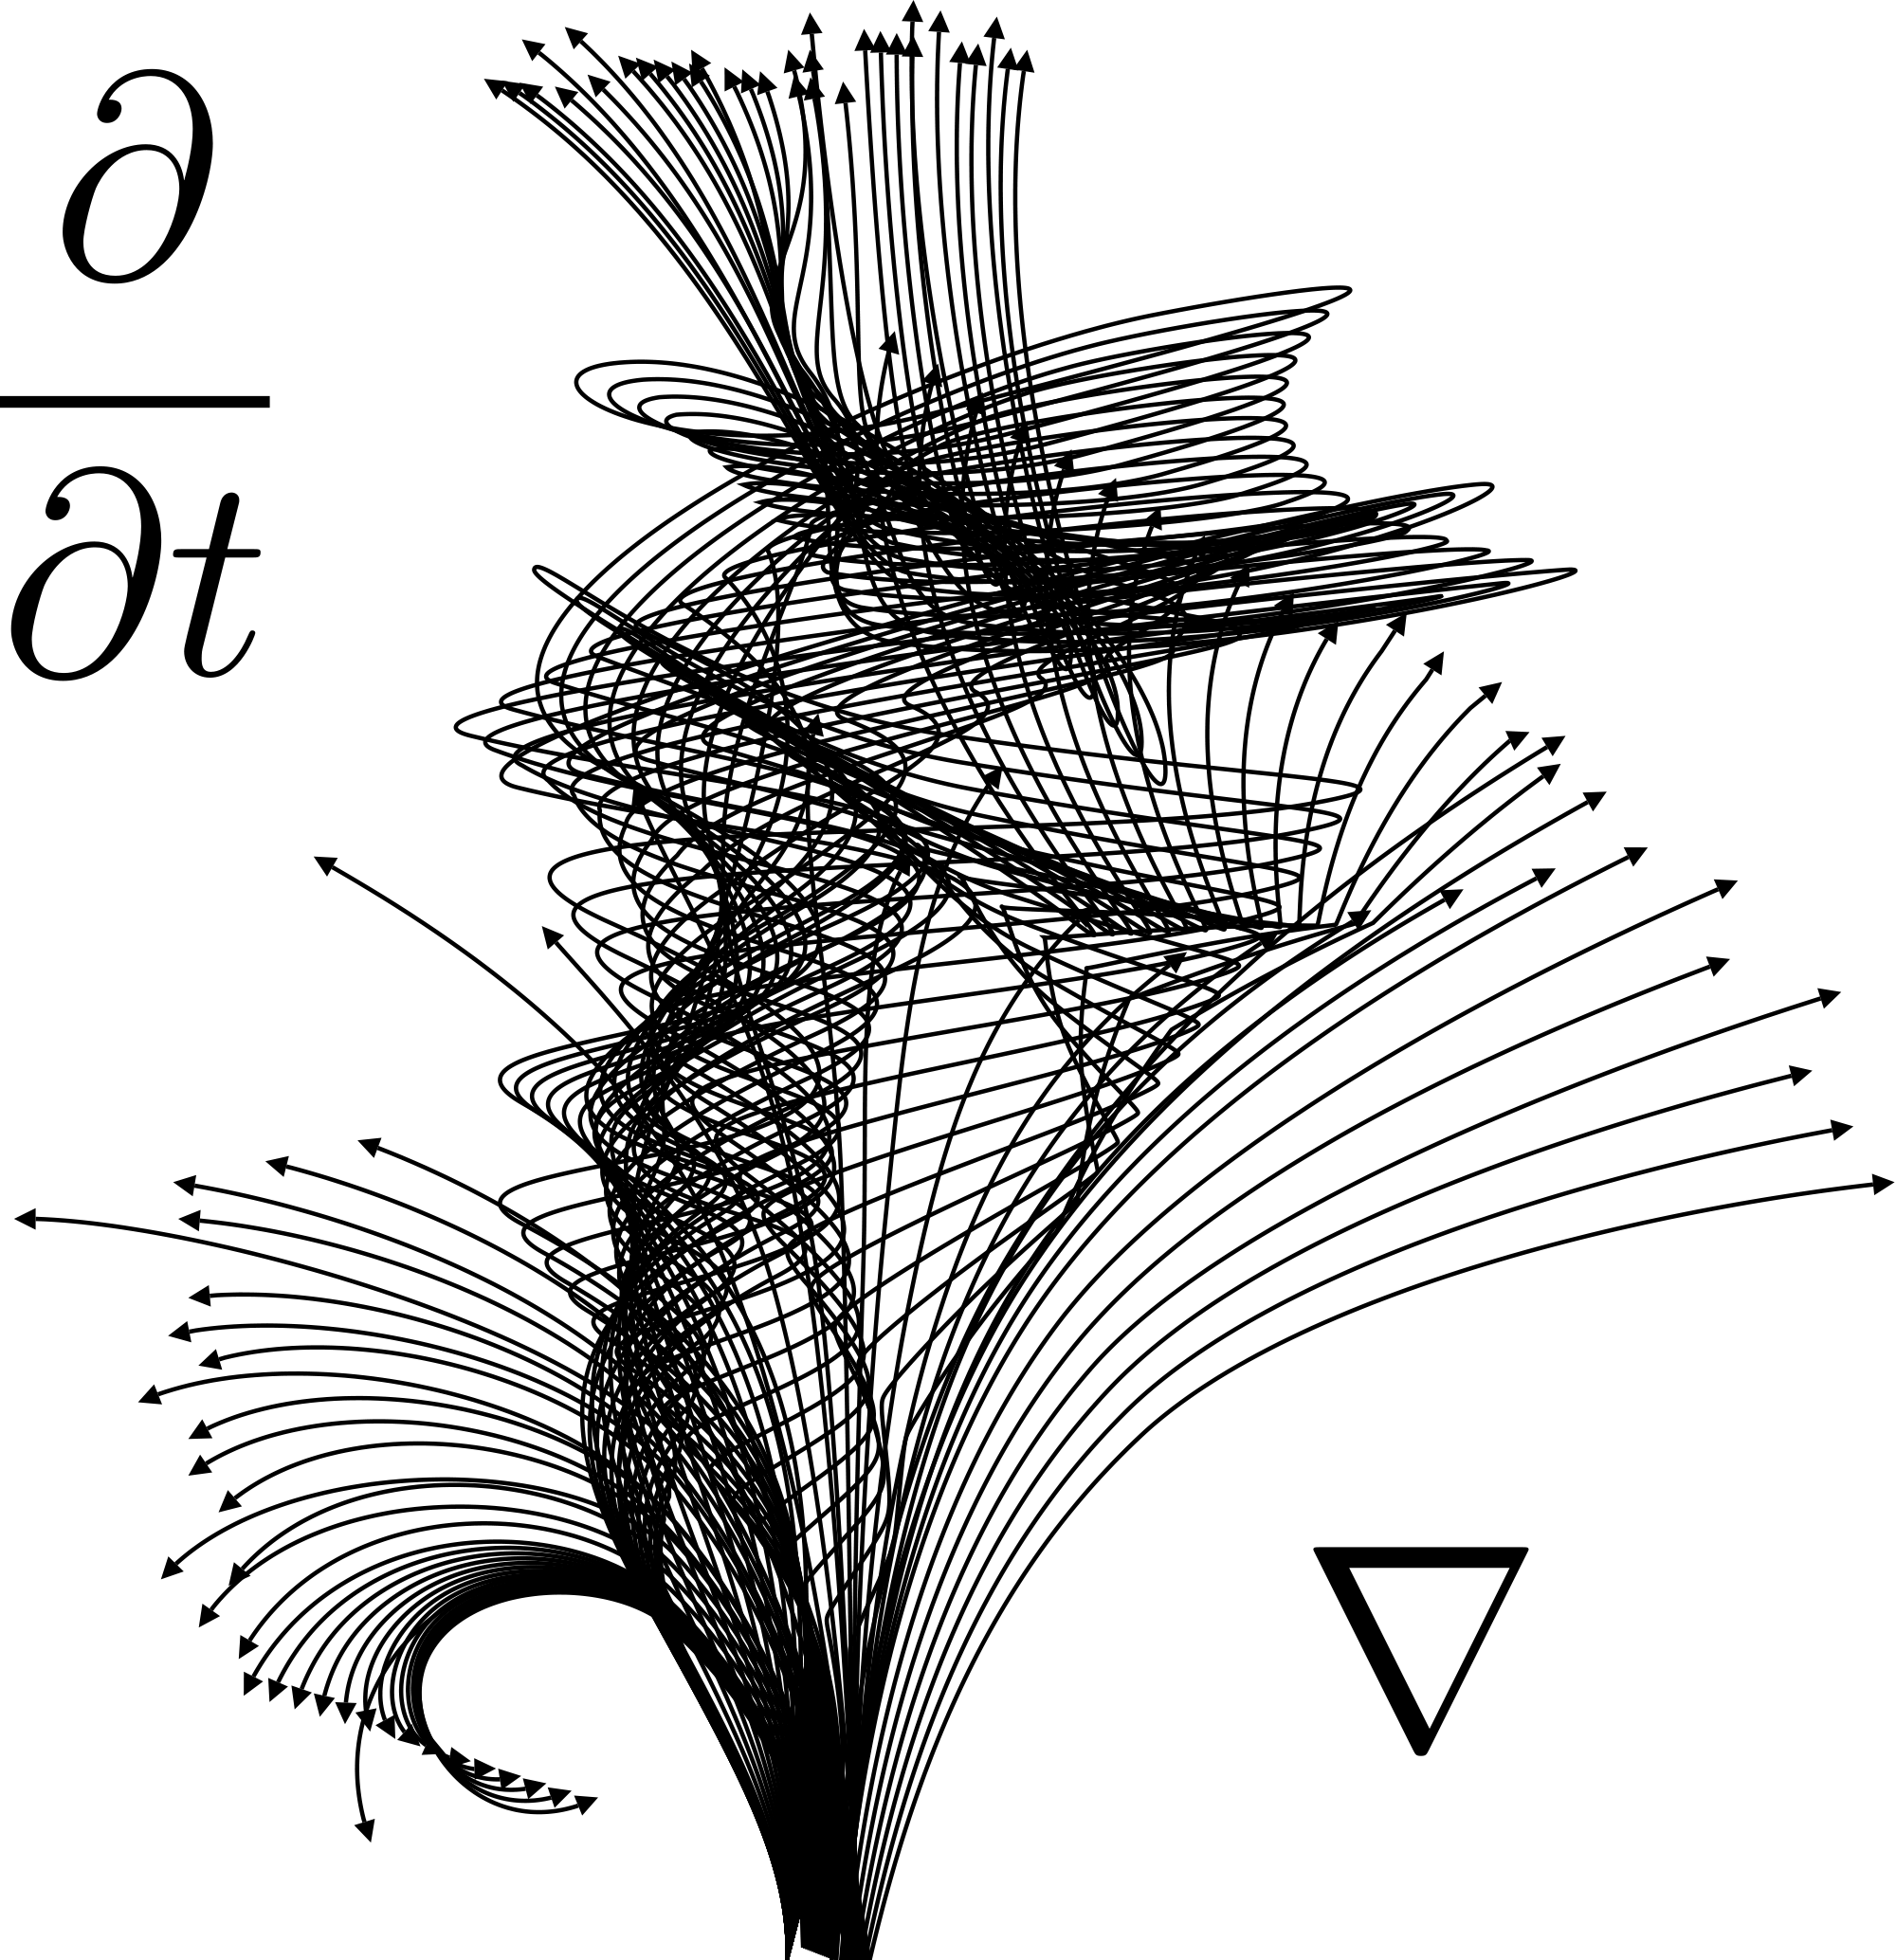
\includegraphics[width=7cm]{Assets/PDE.png}\\[2cm] 
	\center 
	% \quad\\[1.5cm]
	% \textsl{\Large University College Dublin }\\[0.5cm] 
	% \textsl{\large Michale Smurfit Graduate Business School}\\[1.5cm] 
	\makeatletter
	\HRule \\[0.4cm]
	{ \huge \bfseries Quantitative Finance Interview Notes}\\[0.4cm] 
	\HRule \\[2.5cm]

    % \emph{Author:} \textup{Xiaodong Yang}\\[7.5cm]

    {\large \emph{Author:} \textup{\href{https://www.smurfitschool.ie/facultyresearch/phdresearch/phdstudents/xiaodongyang/}{Xiaodong Yang CQF, FRM}}}\\[7.5cm]

	% \begin{minipage}{0.4\textwidth}
	% 	\begin{flushleft} \large
	% 		\emph{Author:}\\
	% 		% \@author 
	% 		\textup{Xiaodong Yang}
	% 	\end{flushleft}
	% \end{minipage}
	% ~
	% \begin{minipage}{0.4\textwidth}
	% 	\begin{flushright} \large
	% 		\emph{Lecturer:} \\
	% 		\textup{Dr Conor Finnegan}
	% 	\end{flushright}
	% \end{minipage}\\[3cm]
	\makeatother
    {\large Detailed information can be found in the README.md file.}\\[0.5cm]
	% {\large An Assignment submitted for the UCAS:}\\[0.5cm]
	% {\large \emph{\href{https://hub.ucd.ie/usis/!W_HU_MENU.P_PUBLISH?p_tag=MODULE&MODULE=ACM30080}{ACM30080 PDEs in Financial Mathematics}}}\\[0.5cm]
	{\large \emph{Last Updated:} \today}\\[2cm] 
	\vfill 
\end{titlepage}



% \maketitle
\newpage% or \cleardoublepage
% \pdfbookmark[<level>]{<title>}{<dest>}
\pdfbookmark[section]{\contentsname}{toc}
\tableofcontents
\thispagestyle{empty}
\pagebreak

\setcounter{page}{1}

\chapter{Probability, Statistics \& Brainteasers}

\section{Probability Foundations (Part A)}

\subsection*{Introduction: Why Probability Dominates Quant Interviews}

Probability is the single most important skill in quant interviews.
A large fraction of questions - brainteasers, logic puzzles, stochastic calculus intuition, derivatives pricing, and risk-neutral reasoning - all reduce to:

\begin{itemize}
    \item computing expectations
    \item understanding conditional probability
    \item analyzing random walks
    \item reasoning under uncertainty
\end{itemize}

Firms use probability questions to test your thinking speed, mathematical maturity, and structural reasoning.

These problems rarely require memorized formulas; instead, they assess whether you can:

\begin{itemize}
    \item break a problem into states
    \item compute conditional paths
    \item identify symmetry
    \item reason recursively
    \item use Markovian structure
\end{itemize}

This section builds the foundation for the more advanced topics later in the chapter.

\subsection*{Probability Axioms (Interview Level)}

Let $(\Omega, \mathcal{F}, \mathbb{P})$ be a probability space. \\
A probability measure satisfies:

\begin{enumerate}
    \item \textbf{Non-negativity:} \\
    $\mathbb{P}(A) \geq 0$
    
    \item \textbf{Normalization:} \\
    $\mathbb{P}(\Omega) = 1$
    
    \item \textbf{Countable additivity:} \\
    If $A_i$ are disjoint, \\
    $\mathbb{P}\left(\bigcup_{i} A_i\right) = \sum_{i} \mathbb{P}(A_i)$
\end{enumerate}

\textbf{Interview expectation:} \\
You never need to formally state these, but many tricky questions rely on:
\begin{itemize}
    \item breaking events into disjoint pieces
    \item checking if events are mutually exclusive
    \item normalizing probabilities
\end{itemize}

\subsection*{Conditional Probability \& Bayes' Rule}

Definition

\begin{equation}
    \mathbb{P}(A \mid B) = \frac{\mathbb{P}(A \cap B)}{\mathbb{P}(B)}
\end{equation}

Bayes' rule

\begin{equation}
    \mathbb{P}(A \mid B) = \frac{\mathbb{P}(B \mid A)\,\mathbb{P}(A)}{\mathbb{P}(B)}
\end{equation}

Total probability

\begin{equation}
    \mathbb{P}(B) = \sum_i \mathbb{P}(B \mid A_i)\,\mathbb{P}(A_i)
\end{equation}

Interview insight:
Most conditional probability questions are solved by:

\begin{enumerate}
    \item Defining states
    \item Applying total probability
    \item Using Bayes' rule for inversion
\end{enumerate}


\subsection*{Classic Interview Example}

\textbf{The Monty Hall Problem}
\ex{}
{
Setup:
You choose 1 of 3 doors; 1 hides a prize.
Host opens another door that definitely has no prize.
Do you switch?

Solution (interview version):

Probability chosen door is correct = 1/3

Probability prize is behind one of the two unchosen doors = 2/3

Host removes one losing option

Switching gives probability = 2/3

Takeaway:
If information is not independent (host has intent), conditional probability changes.

\vspace{1em}

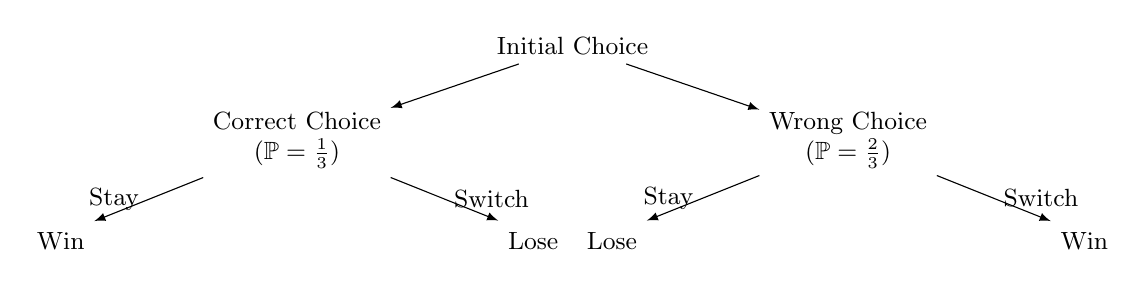
\begin{tikzpicture}[
    >=stealth,
    grow=down,
    level distance=12mm,
    level 1/.style={sibling distance=70mm},   % distance between "Correct" and "Wrong"
    level 2/.style={sibling distance=60mm},   % distance between Stay/Switch leaves
    every node/.style={font=\small, align=center},
    edge from parent/.style={draw, -latex}
]

\node {Initial Choice}
    child {
        node {Correct Choice\\($\mathbb{P} = \tfrac{1}{3}$)}
            child {
                node {\\Win}
                edge from parent node[midway,left] {Stay}
            }
            child {
                node {\\Lose}
                edge from parent node[midway,right] {Switch}
            }
    }
    child {
        node {Wrong Choice\\($\mathbb{P} = \tfrac{2}{3}$)}
            child {
                node {\\Lose}
                edge from parent node[midway,left] {Stay}
            }
            child {
                node {\\Win}
                edge from parent node[midway,right] {Switch}
            }
    };
\end{tikzpicture}
}
\vspace{1em}

\subsection*{Random Variables \& Common Distributions}

Bernoulli
Binary outcome, 0 or 1.
\begin{equation}
    \mathbb{E}[X]=p, \quad \text{Var(X)}=p(1-p)
\end{equation}

Binomial
sum of n Bernoullis.
\begin{equation}
    \text{mean}=np, \quad \text{variance}=np(1-p)
\end{equation}

Poisson (arrivals, jumps)
\begin{equation}
    \mathbb{P}(N_t=k)=\frac{(\lambda t)^ke^{\lambda t}}{k!}
\end{equation}

Key properties:
\begin{itemize}
    \item Independent increments
    \item Stationary increments
    \item Mean = variance = $\lambda t$
\end{itemize}

Interview use cases:

\begin{itemize}
    \item arrival of trades
    \item number of jumps in jump-diffusion
    \item queueing logic
\end{itemize}

Normal Distribution
\begin{equation}
    X\sim N(\mu,\sigma^{2})
\end{equation}

\begin{equation}
    \mathbb{E}[X]=\mu, \quad \mathbb{E}[X^{2}]=\sigma^{2}+\mu^{2}
\end{equation}

\textbf{Expectations, Variance \& Covariance}

Linearity of expectation (critical interview tool):
\begin{equation}
    \mathbb{E}[X + Y] = \mathbb{E}[X] + \mathbb{E}[Y]
\end{equation}


Variance:
\begin{equation}
    \operatorname{Var}(X) = \mathbb{E}[X^2] - (\mathbb{E}[X])^2
\end{equation}

Covariance:
\begin{equation}
    \operatorname{Cov}(X, Y) = \mathbb{E}[XY] - \mathbb{E}[X]\mathbb{E}[Y]
\end{equation}
Correlation:
\begin{equation}
    \rho = \frac{\operatorname{Cov}(X, Y)}{\sigma_X \sigma_Y}
\end{equation}

\subsection*{Common Quant-Interview Expectation Tricks}

Expected value of geometric trials
Until first success:
\begin{equation}
    \mathbb{E}[N]=\frac{1}{p}
\end{equation}

Examples:
\begin{itemize}
    \item die rolls until first 6 $\rightarrow$ 6
    \item coin flips until heads $\rightarrow$ 2
\end{itemize}

Expected value of repeated experiments
if $X_i$ are IID
\begin{equation}
    \mathbb{E}\bigg[\frac{1}{n}\sum_{i=1}^{n} X_i\bigg] = \mathbb{E}[X]
\end{equation}

Symmetry
Many brainteasers are solved instantly by symmetry.

\ex{}{
    Random chord in a circle — probability it is longer than the side of the inscribed triangle?

    Answer depends on chosen definition — interviewers check if you question assumptions.
    }

\subsection*{Random Walks (Discrete)}

Used in:
\begin{itemize}
    \item probability puzzles
    \item gambler’s ruin
    \item Brownian motion intuition
    \item finance models
\end{itemize}

1D symmetric walk
\begin{equation}
    S_{n+1}=S_n+X_n, \quad X_n = \pm 1
\end{equation}

Gambler's Ruin
Probability you hit upper boundary b before lower boundary 0 starting from i: 
Symmetric($p = 0.5$):
\begin{equation}
    \mathbb{P}(\text{hit } b) = \frac{i}{b}
\end{equation}

Asymmetric ($p \neq 0.5$):
\begin{equation}
    \mathbb{P}(\text{hit } b) = \frac{1 - (q/p)^i}{1 - (q/p)^b}
\end{equation}
This appears frequently in quant interviews.


\subsection*{Markov Chains (Interview Level)}

Definition
A process $X_n$ is Markov if:
\begin{equation}
    \mathbb{P}(X_{n+1}=x|X_n\cdots,X_0)=\mathbb{P}(X_{n+1}=x|X_n)
\end{equation}

Used heavily in:
\begin{itemize}
    \item queueing
    \item random walks
    \item credit rating transitions
    \item discretized stochastic models
\end{itemize}

Transition matrix
\begin{equation}
    P = 
    \begin{pmatrix}
    p_{11} & p_{12} \\
    p_{21} & p_{22}
    \end{pmatrix}
\end{equation}

n-step transitions:
\begin{equation*}
    p^{n}
\end{equation*}

\subsection*{Order Statistics (Interview Relevant)}
if you draw $n$ IID samples:
\begin{itemize}
    \item $X_{(1)}=\text{min}$
    \item $X_{(n)}=\text{max}$
\end{itemize}
\ex{}
{
    \begin{equation}
        \mathbb{E}[\text{max}(U_1,\cdots,U_n)]=\frac{n}{n+1}
    \end{equation}
}

\subsection*{Stopping Times (Foundation for Brownian Motion)}
A stopping time $\tau$ satisfies:
\begin{equation*}
    {\tau\le t}\in \mathcal{F}_t
\end{equation*}
\ex{}{
    \begin{itemize}
        \item first time a walk hits $\pm a$
        \item first time volatility exceeds threshold
        \item hitting boundary in Brownian motion (early exercise timing)
    \end{itemize}
}
Interviews rarely ask for formal definition —
they want intuition:
\textbf{“A stopping time is a time at which you stop based only on current information.”}



\section{Deep Conditional Probability, Classic Puzzles \& Core Interview Problems}

\subsection*{Conditional Probability — Core Interview Framework}
Conditional probability is the single most tested concept in quant interviews.
Most puzzles reduce to:
\begin{itemize}
    \item Identify states
    \item Assign base probabilities
    \item Use Bayes’ rule
    \item Compute conditional outcomes
    \item Interpret intuitively
\end{itemize}
Below are advanced forms that often confuse candidates.

\subsection*{The Problem of “Useful vs Useless Information”}
A recurring theme is distinguishing between:

Independent information

Does not change conditional probability
(e.g., rolling a fair die twice)

Dependent information
Massively changes the probability
(e.g., host showing a goat in Monty Hall)

\textbf{Key test in interviews: \\
Always ask yourself: “Does this person KNOW something that influences the outcome?”}

\subsection*{Classic Conditional Probability Puzzle Types}

Type 1: Revealed information
\begin{itemize}
    \item Monty Hall
    \item Cards revealed
    \item Doors opened
    \item Host behaviour
\end{itemize}

Type 2: Random selection vs conditional selection
\begin{itemize}
    \item “You pick a random child and they are a boy…”
vs
    \item “In a family with at least one boy…”
\end{itemize}

Type 3: Biased events
\begin{itemize}
    \item unfair coins
    \item skewed dice
\end{itemize}

Type 4: Symmetry + Bayes
\begin{itemize}
    \item random meeting problems
    \item birthday paradox
    \item dart on a square
\end{itemize}





% \textbf{Advanced Example 1 — The Two-Child Problem (Interview Classic)
% Question}

\subsection*{Interview Classic Problems}

\qprob{The Two-Child Problem}{
    A family has two children.
You meet one of the children randomly, and it is a girl.
What is the probability the other child is a girl?
}

\begin{sol}
    Incorrect intuition:
    “Only two possibilities: GB or GG $\Rightarrow$ 1/2.”

    Correct reasoning:
    Possible equally likely families:
    GG, GB, BG, BB

    Now you meet a random child, and it’s a girl.

    Compute probability of observing “Girl met” in each family:

    GG family → always meet girl (prob = 1)

    GB family → meet girl w.p. 1/2

    BG family → meet girl w.p. 1/2

    BB family → never

    Weighted probabilities:

    GG: 1 × 1

    GB: (1/2) × 1

    BG: (1/2) × 1

    Normalize:
    \begin{align*}
        \mathbb{P}(GG|girl)=\frac{1}{1+\frac{1}{2}+\frac{1}{2}}=\frac{1}{2}
    \end{align*}
    \end{sol}

    % \sol


\qprob{The Drunk Passenger Problem}{
  On a plane with $n$ seats, the first passenger is drunk and picks a random seat. Every subsequent passenger takes their own seat if available; otherwise picks a random available seat. What is the probability the last passenger gets their own seat?  
}
\begin{sol}

Interview solution:
This is a symmetry problem.

The last passenger’s seat is taken only if:
\begin{itemize}
    \item the drunk passenger picks their seat first
    \item OR someone else random-picks it later
\end{itemize}

The shocking fact:

Once the drunk picks a wrong seat, the problem resets with two “special” seats:

\begin{itemize}
    \item seat 1
    \item seat $n$ (last passenger)
\end{itemize}

Every time someone is forced to pick randomly, the choice is only between the first and last seats eventually.

Thus:
\begin{align*}
    \mathbb{P}(\text{last person gets own seat})=\frac{1}{2}
\end{align*}

\end{sol}

\qprob{Random Meeting Problem}
{
  Two friends agree to meet between 0 and 1 hour.
Each arrives at a random time uniformly and waits 15 minutes.
What is the probability they meet?  
}
\begin{sol}
    Solution via geometry

You meet if:
\begin{align*}
    |X-Y|<0.25
\end{align*}

In the unit square, the “meeting band” is:
\begin{align*}
\begin{aligned}
\text{Area} 
&= 1 - 2 \times (\text{triangles each with side } 0.75) \\
&= 1 - 2 \times \frac{1}{2} (0.75)^2 \\
&= 1 - 0.5625 \\
&= 0.4375.
\end{aligned}
\end{align*}

\centering
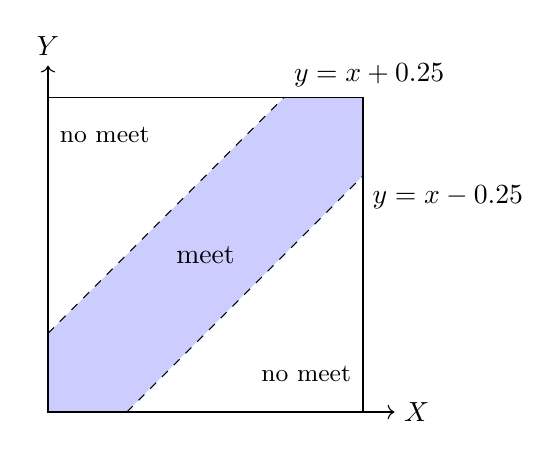
\begin{tikzpicture}[scale=4]
    
  % Axes
  \draw[->] (0,0) -- (1.1,0) node[right] {$X$};
  \draw[->] (0,0) -- (0,1.1) node[above] {$Y$};

  % Shade the whole square first
  \fill[blue!20] (0,0) rectangle (1,1);

  % Cut out the two "no–meet" triangles
  \fill[white] (0,1) -- (0,0.25) -- (0.75,1) -- cycle;   % top-left
  \fill[white] (1,0) -- (0.25,0) -- (1,0.75) -- cycle;   % bottom-right

  % Border of unit square
  \draw (0,0) rectangle (1,1);

  % Meeting band boundaries |X-Y| = 0.25
  \draw[dashed] (0,0.25) -- (0.75,1) node[above right] {$y=x+0.25$};
  \draw[dashed] (0.25,0) -- (1,0.75) node[below right] {$y=x-0.25$};

  % Optional region labels
  \node at (0.5,0.5) {meet};
  \node at (0.18,0.88) {\small no meet};
  \node at (0.82,0.12) {\small no meet};
\end{tikzpicture}


\end{sol}

\qprob{Harder Version — Different Wait Times}
{
    Two friends agree to meet between time 0 and 1 hour.
    \begin{itemize}
        \item Friend A arrives uniformly on $[0,1]$ and waits $a$ hours
        \item Friend B arrives uniformly on $[0,1]$ and waits $b$ hours
    \end{itemize}
    (where $0<a,b<1.$)

    What is the probability they meet?
}

\begin{sol}
    
Two friends arrive at times $X$ and $Y$ on $[0,1]$.
Friend A waits $a$ hours and B waits $b$ hours.  
They meet exactly when the arrival intervals overlap, which is
$-b \le Y-X \le a$.  
For uniform arrivals this is the area of a diagonal band in the unit square.
You remove two no-meeting triangles of area $\tfrac12(1-a)^2$ and
$\tfrac12(1-b)^2$, so  
\[
\mathbb{P}(\text{meet}) = 1 - \frac{(1-a)^2 + (1-b)^2}{2}.
\]
For arbitrary arrival distributions you integrate the joint density over that
band.

\centering
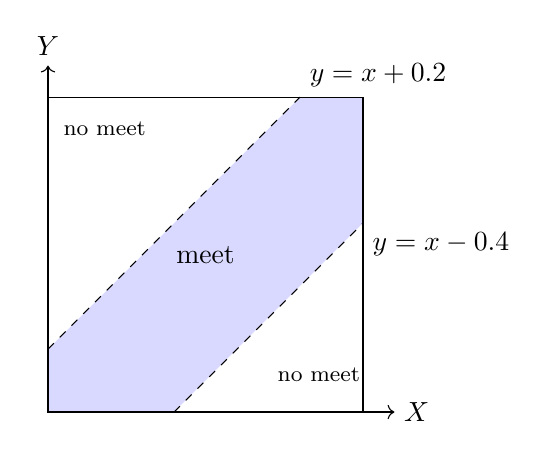
\begin{tikzpicture}[scale=4]
  % parameters (change these if you like)
  \def\a{0.2}  % A's wait time
  \def\b{0.4}  % B's wait time

  % Axes
  \draw[->] (0,0) -- (1.1,0) node[right] {$X$};
  \draw[->] (0,0) -- (0,1.1) node[above] {$Y$};

  % Base square
  \fill[blue!15] (0,0) rectangle (1,1);   % background

  % Cut out non-meeting triangles (white)
  % Top-left: bounded by y=1, x=0, line y = x + a
  \fill[white] (0,1) -- (0,\a) -- (1-\a,1) -- cycle;

  % Bottom-right: bounded by y=0, x=1, line y = x - b
  \fill[white] (1,0) -- (\b,0) -- (1,1-\b) -- cycle;

  % Draw outer square border
  \draw (0,0) rectangle (1,1);

  % Meeting band boundaries: y = x + a and y = x - b
  \draw[dashed] (0,\a) -- (1-\a,1) node[above right] {$y=x+\a$};
  \draw[dashed] (\b,0) -- (1,1-\b) node[below right] {$y=x-\b$};

  % Labels
  \node at (0.5,0.5) {meet};
  \node[font=\footnotesize] at (0.18,0.9) {no meet};
  \node[font=\footnotesize] at (0.86,0.12) {no meet};
\end{tikzpicture}

\end{sol}

\qprob{The Birthday Paradox}
{
    How many people are needed so that the probability of at least one shared birthday is 50\%?
}

\begin{sol}
    \[
    \mathbb{P}(\text{no match})=\frac{365}{365}\times \frac{364}{365}\times\cdots \times \frac{365-n+1}{365}
    \]

    Set equal to $\frac{1}{2}$, solve numerically.
\end{sol}

\qprob{The Balls \& Bins Problem}
{
    Throw $n$ balls into $n$ bins independently and uniformly.
What is the expected number of empty bins?

}

\begin{sol}
    For a given bin:
    \[
    \mathbb{P}(\text{empty})=\bigg(1-\frac{1}{n}\bigg)\approx e^{-1}
    \]

    So:
    \[\mathbb{E}[\text{empty bins}]=ne^{-1}\]
\end{sol}

\subsection*{Deep Dive: Gamma(Shape, Scale)}

Gamma distributions show up in:
\begin{itemize}
    \item waiting times
    \item variance-gamma models (used in quant finance)
    \item Bayesian statistics
    \item mixture models
\end{itemize}

Properties
\[
X\sim \Gamma(k,\theta)\\
\]
\[
\mathbb{E}[X]=k\theta, \quad \text{Var}(X)=k\theta^{2}
\]
Interviews often test “identify the right distribution” when:
\begin{itemize}
    \item time between jumps
    \item sum of exponential variables
\end{itemize}

\subsection*{Quant Interview Questions}

\qprob{}{
    Roll a die repeatedly. What is the expected number of rolls until you see the sequence 1–1 (two ones in a row)?
}

\begin{sol}
    
    This is a Markov chain with 2 states:

    $S_0$ = no previous 1

    $S_1$ = last roll was 1

Solve linear equations:
$\text{Expected rolls} = 36/11 \approx 3.27$

\end{sol}

\qprob{}{
    What is the probability that the maximum of two independent Uniform(0,1) variables exceeds 0.8?
}

\begin{sol}
    
    $1-0.8^2=0.36$

\end{sol}

\qprob{}{
    A fair coin is tossed until heads. Expected tosses?
}

\qprob{}{
    A box has 3 white and 2 black balls. Two are drawn without replacement. Probability both white?
}

\qprob{}{
    What is the expected value of the maximum of 3 IID Uniform(0,1) variables?
}

\qprob{}{
    What is $\mathbb{E}[X|X>1]$ for exponential rate 1?
}

\qprob{}{
    Draw a random point in a unit square. Probability $x+y<1$?
}

\qprob{}{
    Flip a fair coin 10 times. Probability of exactly 5 heads?
}

\qprob{}{
    If two stocks have correlation $\rho$, what is the covariance?
}

\qprob{}{
    Probability that Poisson($\lambda$) variable is even?
}


\subsection*{Brainteasers}

\bts{}{
    The Light Switch Puzzle (Short Version)
}

\sol

Turn switch A on for 5 minutes

Turn off A, turn on B

Enter room:

Light on $\to$ B

Light off but warm $\to$ A

Light off and cold $\to$ C

\bts{}{
    Two Ropes Burning (45 Minutes)
}

\sol

Burn Rope 1 at both ends

Burn Rope 2 at one end

When Rope 1 finishes (30 min), light Rope 2 other end

Rope 2 burns remaining 15 min

Total = 45 min

\bts{}{
    100 Lockers
}

\sol

Only lockers with square numbers stay open
(because toggled odd number of times).

\bts{}{
    Find Heavier Ball With Two Weighings
}

\sol

Use a $3\times3\times3$ splitting; identify remainder group recursively.
\bts{}{
    Farmer, Wolf, Sheep, Cabbage
}
\sol
Sheep first, return alone, wolf next, bring back sheep, cabbage over, return empty, sheep last.

\bts{}{
    Mislabeled Bags
}
\sol
Draw one fruit from the “mixed” label (which must be wrong).
Deduce all labels.
\bts{}{
    Ants on a Stick
}
\sol
Expected time until fall depends on boundaries and speeds—
but direction doesn't matter: ants can be treated as ghosts passing through.

\bts{}{
    12 Coins, One Fake (Unknown Heavier/Light)
}
\sol 
Three weighings $\to$  ternary decision tree (27 leaves $\ge$ 24 possibilities).

\bts{}{
    The Hotel Bill Problem
}
\sol
(paradox with missing \$1; resolve misdirection)

\bts{}{
    Monty Hall Variation
}
\sol
Stay vs switch when multiple goats opened $\to$ generalize to $(n-1)/n$ win rate when switching.\newline


\section{Advanced Probability, Order Statistics, More Interview Questions, and More Brainteasers}

\subsection*{Advanced Probability: Decomposition, Law of Total Expectation}
\subsection*{Advanced Bayes Rule Use-Cases in Interviews}
\subsection*{Order Statistics (Deep Dive)}
\subsection*{Extreme Value Behavior (Useful for your actual PhD research)}
\subsection*{Advanced Interview Questions (20 More)}
\subsection*{Brainteasers (10 More, With Solutions)}


\subsection*{Advanced Distributions for Quant Interviews + Heavy Tails + Extreme Value Theory}

\subsection*{Lognormal Distribution - Core of Quant Finance}
\subsection*{Student-t Distribution - Why It Matters for Quant Jobs}
\subsection*{Laplace Distribution - The “Double Exponential”}
\subsection*{Mixture Models (Gaussian Mixtures)}
\subsection*{Extreme Value Theory (EVT) - Connection to My Research}
\subsection*{Maximum Domain of Attraction - When Extremes Behave Nicely}
\subsection*{Advanced: Lognormal Mixture = Heavy Tail}
\subsection*{20 Advanced Probability Interview Questions (With Solutions)}
\subsection*{10 Advanced Brainteasers}

\section{Brownian Motion, Scaling Limits, Quadratic Variation, Hitting Times, Jensen's Inequality}

\subsection*{From Random Walk to Brownian Motion (Central Insight)}
\subsection*{Definition of Brownian Motion (Interview Level)}
\subsection*{Crucial Property: Quadratic Variation}
\subsection*{Stopping Times - Deepening the Intuition}
\subsection*{Hitting Times of Brownian Motion}
\subsection*{Reflection Principle (Very Common in Interviews)}
\subsection*{Scaling Property of Brownian Motion}
\subsection*{Jensen's Inequality (Very Important)}
\subsection*{Optional Stopping Theorem (Intuition Only)}
\subsection*{10 Bridge to Stochastic Calculus (Setting Up Chapter 2)}
\subsection*{20 Advanced Interview Questions (Continuous-Time \& Theory)}
\subsection*{10 More Brainteasers}


% \section{STATISTICS, ESTIMATION \& SAMPLING THEORY}

\section{Foundations of Estimation, Bias, Variance, MSE, and Sampling}
\subsection*{Introduction: Why Statistics is Critical in Quant Interviews}
\subsection*{Point Estimation Theory}
\subsection*{Common Estimators Every Quant Must Know}
\subsection*{Method of Moments (MoM)}
\subsection*{Maximum Likelihood Estimation (MLE)}
\subsection*{Large Sample (Asymptotic) Theory}
\subsection*{Confidence Intervals (CI)}
\subsection*{Hypothesis Testing Overview}
\subsection*{Sampling Distributions}
\subsection*{Covariance Matrices \& Portfolio Statistics}
\subsection*{Shrinkage Estimators}
\subsection*{20 Statistics Interview Questions (With Solutions)}
\subsection*{10 Statistics Brainteasers}

% \section{BRAINDTEASERS \& QUANT PUZZLES}
\section{Regression, OLS, HAC Standard Errors, Multicollinearity, Predictive Modeling \& Interview Questions}
\subsection*{Introduction: Why Regression is Critical for Quants}
\subsection*{OLS Basics}
\subsection*{Assumptions for Classical OLS (Gauss-Markov)}
\subsection*{OLS Variance and Standard Errors}
\subsection*{$R^2$ and Adjusted $R^2$}
\subsection*{Multicollinearity}
\subsection*{Heteroskedasticity and White Standard Errors}
\subsection*{Autocorrelation \& HAC / Newey-West Standard Errors}
\subsection*{Forecasting vs Inference}
\subsection*{Model Overfitting \& Underfitting}
\subsection*{Regularization in Regression (High-Level)}
\subsection*{Logistic Regression}
\subsection*{20 Regression Interview Questions (with Answers)}
\subsection*{10 Regression Brainteasers}

\section{Time-Series Models, Forecasting, Stationarity, Cointegration, Kalman Filter, GARCH \& Interview Questions}
\subsection*{Introduction: Why Time Series Matters in Quant Interviews}
\subsection*{Stationarity - The Foundational Concept}
\subsection*{Autocorrelation Function (ACF) \& Partial ACF (PACF)}
\subsection*{AR(1) Model}
\subsection*{MA(1) Model}
\subsection*{ARMA Models}
\subsection*{ARIMA and Differencing}
\subsection*{Random Walks (Very Common in Finance)}
\subsection*{Unit Roots \& ADF Test (Augmented Dickey-Fuller Test)}
\subsection*{Cointegration - Super Important for Quant Interviews}
\subsection*{Vector Autoregressions (VAR)}
\subsection*{State-Space Models \& Kalman Filter}
\subsection*{ARCH \& GARCH - Volatility Clustering}
\subsection*{20 Time-Series Interview Questions (With Solutions)}
\subsection*{10 Time-Series Brainteasers}

\section{Machine Learning for Quants}
\subsection*{Introduction: Why Machine Learning Matters in Quant Interviews}
\subsection*{Supervised Learning Overview}
\subsection*{Bias-Variance Tradeoff (Most Important ML Interview Concept)}
\subsection*{Cross-Validation (CV)}
\subsection*{Regularization Methods}
\subsection*{Tree-Based Methods}
\subsection*{Ensemble Methods: Bagging, Random Forest, Boosting}
\subsection*{Support Vector Machines (SVM)}
\subsection*{K-Nearest Neighbors (kNN)}
\subsection*{Clustering Methods: K-Means, Hierarchical, SOM}
\subsection*{Principal Component Analysis (PCA)}
\subsection*{Neural Networks: Foundation for LSTM \& Deep Learning}
\subsection*{Time-Series ML Challenges}
\subsection*{Feature Engineering}
\subsection*{20 Machine Learning Interview Questions (With Answers)}
\subsection*{10 Machine Learning Brainteasers}

\section{Brainteaser Compendium}

\newpage

\chapter{Derivatives, Greeks, Models \& Stochastic Calculus}


\section{Black-Scholes-Merton Derivations}

This section is one of the MOST important parts of quantitative finance. \\
Top firms LOVE asking:
\begin{itemize}
    \item “Derive Black–Scholes.”
    \item “Why does $\mu$ disappear?”
    \item “Explain risk-neutral pricing.”
    \item “Explain delta hedging.”
    \item “What is replication?”
    \item “What is the intuition behind Girsanov?”
\end{itemize}
You must know multiple derivations because different interviewers prefer different perspectives.


\subsection*{Why Does Risk-Neutral Pricing Work?}

This is a COMMON interview question.\\
\textbf{Key Idea}\\
We are NOT saying investors are risk-neutral.\\
Instead:
\begin{itemize}
    \item hedging removes risk
    \item therefore derivative price must equal replication cost
    \item under no-arbitrage, there exists equivalent martingale measure $\mathbb{Q}$ 
\end{itemize}
Under $\mathbb{Q}$: all discounted tradable assets are martingales.

\subsection*{Derivation 4: Feynman-Kac Representation}

The PDE:

\[V_t+\mathcal{L}V-rV=0\]
with terminal payoff:

\[V(S,T)=\Phi(S)\]
has solution:

\[V(S,t)=E^{\mathbb{Q}}[e^{-r(T-t)}\Phi(S_T)]\]
This is the Feynman-Kac theorem. \\
It connects:
\begin{itemize}
    \item PDEs
    \item stochastic calculus
    \item expectations
    \item pricing theory
\end{itemize}
This is VERY important for advanced quant interviews.

\subsection*{}

\subsection*{}

\subsection*{}

\subsection*{}

\section{Greeks}
\section{Trees, Monte Carlo, PDE \& FEM}
\section{Stochastic calculus}
\section{Models beyond BSM}
\section{Hedging \& replication}
\section{Derivatives interview Q\&A}
% \section{}

\newpage

% \section{}


\chapter{Coding, Math, Linear Algebra \& Technical Computing}

\section{Coding Fundamentals for Quants (Python + C++)}

\section{Math Essentials}

\section{Coding + Probability}

\section{Practical Quant Engineering}

\section{Full Coding Interview Problems}

\newpage

\chapter{Numerical Methods, C++, \& HFT-Style Algorithms}

\section{Numerical Methods in Quant Finance}

\subsection*{Root Finding}

TextTextTextTextTextTextTextTextTextTextTextTextTextText

\subsection*{Numerical Integration}
\subsection*{Finite Difference Methods for PDEs}
\subsection*{Monte Carlo Methods (Advanced)}
\subsection*{Numerical Linear Algebra}

\section{C++ for Quants (Low-Latency Coding)}

\subsection*{C++ Basics for Speed}
\subsection*{Memory \& Cache Optimization}
\subsection*{Efficient Data Structures}
\subsection*{Exception Safety, Error Handling}
\subsection*{Build optimization (O2/O3, LTO, PGO)}

\section{High-Frequency Trading (HFT) Algorithms \& Data Structures}

\subsection*{Order Book Modeling}
\subsection*{Microstructure Models}
\subsection*{HFT Data Structures}
\subsection*{Latency-Sensitive Coding}
\subsection*{Simulating Order Books}

\section{Numerical Option Pricing}

\subsection*{Black–Scholes (Analytic and Numeric)}
\subsection*{Binomial \& Trinomial Trees}
\subsection*{PDE Methods}
\subsection*{Heston \& SV Models}
\subsection*{Jumps (Merton, Bates)}

\section{Probabilistic \& Statistical Tools for HFT}

\subsection*{Poisson \& Hawkes Processes}
\subsection*{Microprice \& Queue Estimation}
\subsection*{Market Impact Models}

\section{Coding Interview Problems (C++ / Python)}

\newpage

\chapter{Portfolio Optimization, Execution, and Systematic Strategy Design}

\section{Signal Construction \& Alpha Modeling}
\subsection*{Types of signals}
\subsection*{Forecasting returns}
\subsection*{Combining forecasts}
% \subsection*{}
% \subsection*{}

\section{Position Sizing \& Risk Constraints}
% \subsection*{}
% \subsection*{}
% \subsection*{}
% \subsection*{}
% \subsection*{}

\section{Portfolio Optimization (Modern Quant Version)}
\subsection*{Classical MPT failure modes}
\subsection*{Robust optimization}
\subsection*{Shrinkage covariance matrices}
\subsection*{Black-Litterman}
\subsection*{Hierarchical Risk Parity (HRP)}
\subsection*{Convex optimization}

\section{Statistical Arbitrage \& Pairs Trading}
\subsection*{Mean-reversion signals}
\subsection*{Z-score normalization}
\subsection*{Kalman-filter pairs (time-varying beta)}
\subsection*{Cointegration}
\subsection*{Spread modeling}
\subsection*{Execution of stat-arb portfolios}

\section{Backtesting \& Simulation Frameworks}
\subsection*{Event-driven backtesting}
\subsection*{Slippage models}
\subsection*{Market impact adjustment}
\subsection*{Realistic fill assumptions}
\subsection*{Latency effects}
\subsection*{Walk-forward optimization}
\subsection*{Overfitting and leakage avoidance}

\section{Execution Algorithms \& Cost Modeling}
\subsection*{VWAP}
\subsection*{TWAP}
\subsection*{POV (Participation of Volume)}
\subsection*{Adaptive execution}
\subsection*{Implementation shortfall}
\subsection*{Almgren-Chriss optimal execution}
\subsection*{Intraday volume curves}
\subsection*{Venue selection / smart order routing}

\section{Performance Evaluation (Advanced)}
\subsection*{Sharpe / Sortino / Calmar}
\subsection*{Maximum Drawdown}
\subsection*{Alpha decay}
\subsection*{Hit rate}
\subsection*{Return distribution diagnostics}
\subsection*{Tail risk measures (your specialty - LTI!)}
\subsection*{Fama-French attribution}
\subsection*{Strategy capacity}


\section{Production Deployment}
\subsection*{Feature pipelines}
\subsection*{Online retraining}
\subsection*{Monitoring forecast drift}
\subsection*{Latency \& throughput requirements}
\subsection*{Code optimization for production}
\subsection*{Failover and redundancy}
\subsection*{Logging \& audit trail}
% \subsection*{}


\newpage

\chapter{Old}

\section{Curated Question Set for Your 6-Week Plan}

\subsection*{Week 1 - Probability Foundations}

Focus: conditional probability, expectations, variance, random walks.

\qprob{}{
    A biased coin has probability $p$ of heads. How many flips do you expect to need to get two consecutive heads?
}

\begin{sol}

    We define the following states based on the current progress toward the goal of "HH" (two consecutive heads):State 0 ($S_0$): We have not yet flipped the coin, or the last flip was a Tail. We have zero consecutive heads.State 1 ($S_1$): Our last flip was a Head. We need one more Head to reach the goal.State 2 ($S_2$): We have achieved two consecutive heads. This is our stopping state.

    Let $E_0$ be the expected number of additional flips needed to reach $S_2$ starting from $S_0$, and $E_1$ be the expected number of additional flips needed starting from $S_1$. We want to find $E_0$.

    From State 0:On the next flip:With probability $p$, we get a Head and move to $S_1$.With probability $q = 1-p$, we get a Tail and stay in $S_0$.The equation is:$$E_0 = 1 + p E_1 + q E_0$$From State 1:On the next flip:With probability $p$, we get a Head and move to $S_2$ (the goal). Since we have reached the goal, the additional flips needed is $0$.With probability $q = 1-p$, we get a Tail and move back to $S_0$.The equation is:$$E_1 = 1 + p(0) + q E_0 = 1 + q E_0$$3. Solving the SystemWe substitute the expression for $E_1$ into the equation for $E_0$:$$E_0 = 1 + p(1 + q E_0) + q E_0$$$$E_0 = 1 + p + pq E_0 + q E_0$$Now, group the $E_0$ terms on one side:$$E_0 - pq E_0 - q E_0 = 1 + p$$$$E_0 (1 - q(p + 1)) = 1 + p$$Substitute $q = 1-p$ into the term $(1 - q(p+1))$:$$1 - (1-p)(1+p) = 1 - (1 - p^2) = p^2$$So the equation becomes:$$E_0 (p^2) = 1 + p$$$$E_0 = \frac{1+p}{p^2}$$Final AnswerThe expected number of flips to get two consecutive heads is:$$E = \frac{1+p}{p^2}$$

    \ex{Verification with Common Values}{

    The expected number of flips to get two consecutive heads is:$$E = \frac{1+p}{p^2}$$Verification with Common ValuesFair Coin ($p = 1/2$):$$E = \frac{1 + 0.5}{0.5^2} = \frac{1.5}{0.25} = 6 \text{ flips}$$Certain Heads ($p = 1$):$$E = \frac{1 + 1}{1^2} = 2 \text{ flips}$$(As expected, since every flip is a head, we get HH in exactly 2 flips).

    }

    \end{sol}

\qprob{}{
    A box has red, green, and blue balls. You draw two without replacement. What is the probability the colors match?
}

\begin{sol}
    
    To solve this, we need to look at the total number of ways to pick two balls and how many of those pairs result in a match. Because we aren't given the specific quantities of each color, let’s define them:
    \begin{itemize}
        \item $r$ = Number of red balls
        \item $g$ = Number of green balls
        \item $b$ = Number of blue balls
        \item $n = r + g + b$ (Total number of balls)
    \end{itemize}

    % ### 1. Total Number of Outcomes
    The total number of ways to choose 2 balls out of $n$ without replacement (where order doesn't matter) is given by the combination formula:
    $$\binom{n}{2} = \frac{n(n-1)}{2}$$



    % ### 2. Number of Successful Outcomes (Matching Colors)
    For the colors to match, you must draw either two red balls, two green balls, or two blue balls. We calculate the combinations for each:

    \begin{itemize}
        \item Two Red: $\binom{r}{2} = \frac{r(r-1)}{2}$
        \item Two Green: $\binom{g}{2} = \frac{g(g-1)}{2}$
        \item Two Blue: $\binom{b}{2} = \frac{b(b-1)}{2}$
    \end{itemize}

    The total number of favorable outcomes is the sum of these three:
    $$\text{Favorable} = \frac{r(r-1) + g(g-1) + b(b-1)}{2}$$


    % ### 3. Calculating the Probability
    The probability $P(\text{Match})$ is the ratio of favorable outcomes to total outcomes:

    $$P(\text{Match}) = \frac{\frac{r(r-1) + g(g-1) + b(b-1)}{2}}{\frac{n(n-1)}{2}}$$

    By canceling out the 2 in the denominators, we get the final formula:

    $$P(\text{Match}) = \frac{r(r-1) + g(g-1) + b(b-1)}{n(n-1)}$$



    % ### Alternative Method: Using Individual Probabilities
    You can also think of this as the sum of the probabilities of picking two of each specific color:

    \begin{itemize}
        \item $P(\text{Red and Red})$: $\frac{r}{n} \cdot \frac{r-1}{n-1}$
        \item $P(\text{Green and Green})$: $\frac{g}{n} \cdot \frac{g-1}{n-1}$
        \item $P(\text{Blue and Blue})$: $\frac{b}{n} \cdot \frac{b-1}{n-1}$
    \end{itemize}

    Adding these together gives the same result:
    $$P(\text{Match}) = \frac{r(r-1) + g(g-1) + b(b-1)}{n(n-1)}$$

    \textbf{Note:} If any color has fewer than 2 balls (e.g., $r=1$), the term for that color becomes 0, correctly reflecting that it's impossible to draw a matching pair of that color.

\end{sol}

\qprob{}{
    A random variable $X$ is normally distributed. What is the distribution of $X^2$?
}

\begin{sol}
    
    The distribution of $X^2$ depends entirely on the parameters of the original normal distribution, specifically the mean ($\mu$) and the variance ($\sigma^2$).
    
    1. The Special Case: Standard Normal DistributionIf $X$ is a Standard Normal random variable, meaning $X \sim N(0, 1)$, then $X^2$ follows a Chi-squared distribution with 1 degree of freedom.$$X^2 \sim \chi^2_1$$This is the fundamental definition of the chi-squared distribution.

    2. The Case: $X \sim N(0, \sigma^2)$If the mean is zero but the variance is not 1, we can normalize the variable. Since $(X/\sigma) \sim N(0, 1)$, then:$$(X/\sigma)^2 = \frac{X^2}{\sigma^2} \sim \chi^2_1$$In this case, $X^2$ follows a Scaled Chi-squared distribution, specifically $\sigma^2 \chi^2_1$, which is also a specific case of the Gamma distribution:$$X^2 \sim \text{Gamma}\left(k=\frac{1}{2}, \theta=2\sigma^2\right)$$

    3. The General Case: $X \sim N(\mu, \sigma^2)$If the mean $\mu$ is non-zero, the distribution of $X^2$ becomes more complex.Non-central Chi-squared Distribution: First, we scale the variable to have unit variance: $Z = X/\sigma$. Then $Z \sim N(\mu/\sigma, 1)$.The square of this variable, $(X/\sigma)^2$, follows a Non-central Chi-squared distribution with 1 degree of freedom and non-centrality parameter $\lambda = (\mu/\sigma)^2$.Therefore, for the general case, $X^2$ is a scaled version of a non-central chi-squared variable:$$X^2 \sim \sigma^2 \chi^2_1\left(\lambda = \frac{\mu^2}{\sigma^2}\right)$$



\end{sol}

\qprob{}{
    A stock price follows a random walk with upward probability 0.55. What is the probability it hits +5 before -5?
}

\begin{sol}
    
    This is a classic variation of the Gambler's Ruin problem. We can model the stock price movement as a sequence of independent steps where the price increases by 1 with probability $p$ and decreases by 1 with probability $q = 1 - p$.
    
    1. Variables and ParametersIn this scenario:$p = 0.55$ (Probability of moving up)$q = 1 - 0.55 = 0.45$ (Probability of moving down)$s = 0$ (Starting position)$a = -5$ (Lower boundary)$b = +5$ (Upper boundary)We want to find the probability of reaching $b$ before $a$. To simplify the math, we can shift the coordinates so the process starts at $i = 5$, with a lower bound at $0$ and an upper bound at $N = 10$.
    
    2. The Gambler's Ruin FormulaFor a non-symmetric random walk ($p \neq q$), the probability $P_i$ of reaching the upper boundary $N$ starting from position $i$ is given by:$$P_i = \frac{1 - (q/p)^i}{1 - (q/p)^N}$$
    
    3. CalculationLet's plug in our specific values:The ratio $\frac{q}{p} = \frac{0.45}{0.55} = \frac{9}{11} \approx 0.818$Starting position $i = 5$ (relative to the lower bound)Total distance $N = 10$$$P_5 = \frac{1 - (9/11)^5}{1 - (9/11)^{10}}$$Now, calculating the powers:$(9/11)^5 \approx 0.368$$(9/11)^{10} \approx (0.368)^2 \approx 0.135$Substituting these back into the equation:$$P_5 \approx \frac{1 - 0.368}{1 - 0.135} = \frac{0.632}{0.865}$$$$P_5 \approx 0.7306$$
    
    Final ResultThe probability that the stock hits +5 before it hits -5 is approximately 0.731 (or 73.1\%).Even though the upward bias ($0.55$) seems small, the "drift" significantly stacks the odds in favor of hitting the upper target over a 10-step total range.

\end{sol}

\qprob{}{
    Roll a fair die until you get a 6. What is the expected number of rolls?
}

\begin{sol}
    
    This is a classic problem involving a Geometric Distribution. We are looking for the expected number of trials until the first "success."
    
    1. Defining the ProbabilityFor a fair six-sided die, the probability of rolling a 6 (success) on any given roll is:$$p = \frac{1}{6}$$The probability of rolling anything else (failure) is:$$q = 1 - p = \frac{5}{6}$$
    
    2. The Expected Value FormulaFor a geometric distribution, the expected value $E$ (the average number of trials to get the first success) is given by the reciprocal of the probability of success:$$E = \frac{1}{p}$$
    
    3. CalculationPlugging in our value for $p$:$$E = \frac{1}{1/6} = 6$$

    Why is it $1/p$? (The Intuitive Proof)

    \begin{proof}
        If you aren't familiar with the formula, you can derive it using a simple recursive logic similar to the "consecutive heads" problem:Let $E$ be the expected number of rolls.On the first roll, you get a 6 with probability $1/6$. If this happens, you are done (1 roll).You fail to get a 6 with probability $5/6$. If this happens, you have "wasted" one roll and are essentially back at the beginning. You still expect to need $E$ more rolls.The equation looks like this:$$E = \frac{1}{6}(1) + \frac{5}{6}(1 + E)$$$$E = \frac{1}{6} + \frac{5}{6} + \frac{5}{6}E$$$$E = 1 + \frac{5}{6}E$$Subtract $\frac{5}{6}E$ from both sides:$$\frac{1}{6}E = 1$$$$E = 6$$
    \end{proof}

    Final Result
    You expect to need 6 rolls to get a 6.

    It makes intuitive sense: if something happens 1 out of every 6 times on average, you'd expect to wait about 6 times for it to occur!

\end{sol}



\qprob{}{
    You flip a fair coin 10 times. What’s the probability of exactly 5 heads?
}

\begin{sol}



\end{sol}

\qprob{}{
    if $X\sim \text{Possion}(\lambda)$, compute $\text{Var(X)}$ and explain why.
}

\begin{sol}

    To find the probability of exactly 5 heads in 10 flips of a fair coin, we use the Binomial Distribution.
    
    1. Identify the ParametersFor a binomial problem, we need four values:$n = 10$: The total number of trials (flips).$k = 5$: The number of successful outcomes (heads) we want.$p = 0.5$: The probability of success on a single trial.$q = 1 - p = 0.5$: The probability of failure (tails).
    
    2. The Binomial FormulaThe probability of getting exactly $k$ successes in $n$ trials is:$$P(X = k) = \binom{n}{k} p^k q^{n-k}$$
    
    3. Step-by-Step Calculation

    Step A: Calculate the CombinationsFirst, we find how many different ways we can arrange 5 heads in 10 flips. This is "10 choose 5":$$\binom{10}{5} = \frac{10!}{5!(10-5)!} = \frac{10 \times 9 \times 8 \times 7 \times 6}{5 \times 4 \times 3 \times 2 \times 1} = 252$$
    
    Step B: Calculate the ProbabilitiesSince $p$ and $q$ are both $0.5$, the probability part of the formula simplifies:$$p^5 \times q^5 = (0.5)^5 \times (0.5)^5 = (0.5)^{10}$$$$(0.5)^{10} = \frac{1}{1024} \approx 0.0009765625$$
    
    Step C: Multiply Together$$P(X = 5) = 252 \times \frac{1}{1024}$$$$P(X = 5) = \frac{252}{1024} = \frac{63}{256}$$Final ResultThe probability of getting exactly 5 heads in 10 flips is $\frac{63}{256}$, which is approximately 0.2461 or 24.61\%.
    
    Why isn't it 50\%?
    
    It’s a common intuition to think that because heads and tails are equally likely, you should get exactly 5 heads half the time. However, 5 is simply the most likely outcome (the mode); there are many other possibilities (like 4 or 6 heads) that split the remaining probability.

\end{sol}

\qprob{}{
    You observe one normal variable. How do you estimate its variance
}

\begin{sol}

    To estimate the variance of a normal distribution based on a single observation ($n=1$), we run into a fundamental mathematical wall: you cannot calculate a sample variance from one data point.However, how you approach this depends on whether you are looking for a standard statistical estimate or a Bayesian inference.
    
    1. The Frequentist Reality: It's UndefinedIn classical statistics, the formula for sample variance ($s^2$) requires at least two observations because it measures the "spread" or deviation from a mean.$$s^2 = \frac{\sum (x_i - \bar{x})^2}{n-1}$$If $n=1$, the denominator becomes $1-1=0$. This leads to an undefined result. Intuitively, this makes sense: if you only see one person's height (e.g., 5'10"), you have no way of knowing if everyone else is also exactly 5'10" (zero variance) or if heights range from 4' to 7' (high variance).
    
    2. The Maximum Likelihood ApproachIf you attempt to use Maximum Likelihood Estimation (MLE), which uses $n$ instead of $n-1$, the formula is:$$\hat{\sigma}^2 = \frac{(x_1 - \mu)^2}{1}$$If the mean ($\mu$) is known: You can estimate the variance as the squared deviation from that known mean.If the mean ($\mu$) is unknown: The MLE for the mean is the observation itself ($x_1$). This results in a variance estimate of $(x_1 - x_1)^2 = 0$. This is a "biased" estimate and almost certainly incorrect, as it assumes the population has no spread.
    
    3. The Bayesian Approach (The "Workaround")If you absolutely must have an estimate from one data point, you use Prior Knowledge. You don't start from zero; you start with an assumption about what the variance might be (a "Prior Distribution").
    
    Prior: You assume the variance follows an Inverse-Gamma distribution (the conjugate prior for variance).
    
    Observation: You see $x_1$.
    
    Posterior: You update your belief. The single observation "pulls" the prior toward the value of $(x_1 - \mu)^2$.

    The Bottom Line: With $n=1$, you can't measure "difference" because there is nothing to differ from. You either need more data, a known mean, or a strong prior assumption.

\end{sol}



\subsection*{WEEK 2 — Brainteasers \& Logic}

From Chapter 8 (rewritten)

\qprob{}{
    You have 3 light switches and 1 bulb in a separate room. How do you determine which switch controls the bulb with one visit?
}

\sol ss

\qprob{}{
    You have two ropes. Each burns in exactly one hour but not at a constant rate. How do you measure 45 minutes?
}

\qprob{}{
    You stand in front of 100 closed lockers. You toggle every k-th locker on pass k. Which lockers stay open?
}

\qprob{}{
    A man pushes his car to a hotel and is immediately bankrupt. Explain.
}

\qprob{}{
    You are given 8 balls; one is heavier. How do you find the heavy one using two weighings?
}


\qprob{}{
    You need to divide 8 liters into 2 and 6 using only a 5-L and 3-L container.
}


\qprob{}{
    You and another person each draw a random real number in (0,1). You choose separately whether to select or pass. Strategy?
}


% \qprob{Two-Child Problem}{
% A family has two children. You meet one child randomly, and it is a girl.
% What is the probability the other child is also a girl?
% }

\subsection*{WEEK 3 — Options \& Derivatives}

Based on Chapters 2.2.1, 2.2.2, 2.2.3, 2.2.4

\qprob{}{
    Re-derive the Black–Scholes PDE using delta hedging.
}

\qprob{}{
    Explain intuitively why Gamma is always positive for calls and puts.
}

\qprob{}{
    Why does Vega always decrease as time to maturity approaches zero?
}

\qprob{}{
    Construct a replicating portfolio for a binary option.
}

\qprob{}{
    Explain why call prices increase with volatility.
}

\qprob{}{
    How can you price an Asian option with Monte Carlo?
}

\qprob{}{
    Why is implied volatility skewed in equity index options?
}


\qprob{}{
    Explain the intuition behind local volatility vs stochastic volatility.
}

\qprob{}{
    Show how to approximate Delta and Gamma numerically.
}


\subsection*{WEEK 4 — Math + Stochastic Processes}

Based on Chapters 3 \& 6

\qprob{}{
    State and apply Itô's lemma to $X_t=S_t^2$.
}

\qprob{}{
    A Brownian motion hits level 1. What is the distribution of the hitting time?
}

\qprob{}{
    Solve the SDE $dX_t=\mu X_tdt+\sigma dW_t$.
}

\qprob{}{
    Show that GBM is lognormal.
}

\qprob{}{
    Compute $\mathbb{E}[\int_{0}^{T}W_tdt]$ and $\text{Var}[\int_{0}^{T}W_tdt]$.
}

\qprob{}{
    If two Brownian motions have correlation $\rho$, write a simulation scheme.
}

\qprob{}{
    Does a Poisson process have independent increments? Explain.
}

\qprob{}{
    Interpret the drift and volatility of the OU process in simple language.
}

\subsection*{WEEK 5 — Coding \& Numerical Methods}

Based on Chapters 5 \& 7

\qprob{}{
    Write a Monte Carlo simulation for GBM.
}

\qprob{}{
    Implement a function to compute the sample covariance matrix.
}

\qprob{}{
    Implement finite-difference approximation of Delta.
}

\qprob{}{
    Price a European option using variance reduction (Antithetic).
}

\qprob{}{
    Simulate a correlated Brownian motion vector.
}

\qprob{}{
    Implement a simple trinomial tree.
}

\qprob{}{
    Price a digital call with Monte Carlo + control variates.
}

\qprob{}{
    Compute PCA of a covariance matrix using NumPy.
}

\subsection*{WEEK 6 — Mock Interviews + Soft Questions}

Based on Chapters 1 \& 9

\textbf{Technical questions}

\qprob{}{
    Explain your research in 30 seconds.
}

\qprob{}{
    What is tail risk?
}

\qprob{}{
    What is the intuition behind volatility risk premium?
}

\qprob{}{
    How does implied skew relate to crash risk?
}

\qprob{}{
    Why are index options negatively skewed?
}

\qprob{}{
    Compare your LTI measure to existing tail measures (BT11Q).
}


\textbf{Soft questions}

\qprob{}{
    Describe a time you had to debug a complex model.
}

\qprob{}{
    How would your supervisor describe you?
}

\qprob{}{
    What is your biggest weakness in quant finance?
}

\section{Upgraded version}




\section{New Problems}





\subsection*{Deep Conditional Probability, Classic Puzzles \& Core Interview Problems}



\textbf{Quant Interview Questions}










% \textbf{Advanced Example 1 — The Two-Child Problem (Interview Classic)}












\vspace{1em}

% Optional: citation formatted by natbib
% \textbf{Full Citation:} \\
% \citep{yourbibkeyhere}





















\bibliographystyle{agsm}
% \bibliographystyle{jfqa}
\clearpage
\addcontentsline{toc}{section}{References} 
\bibliography{ref}
% \bibliographystyle{jfqa}
% \bibliography{ref}

% \clearpage
% \addcontentsline{toc}{section}{References}
% \bibliographystyle{jfqa}   % or agsm, or elsarticle-harv, etc.
% \bibliography{ref}


\end{document}
